\documentclass{article}
\usepackage{tikz}
\usepackage{amsmath,amssymb,amsfonts}
\usepackage{xcolor}

\newcommand{\ol}{\overline}

\newcommand{\mc}{\mathcal}

\begin{document}

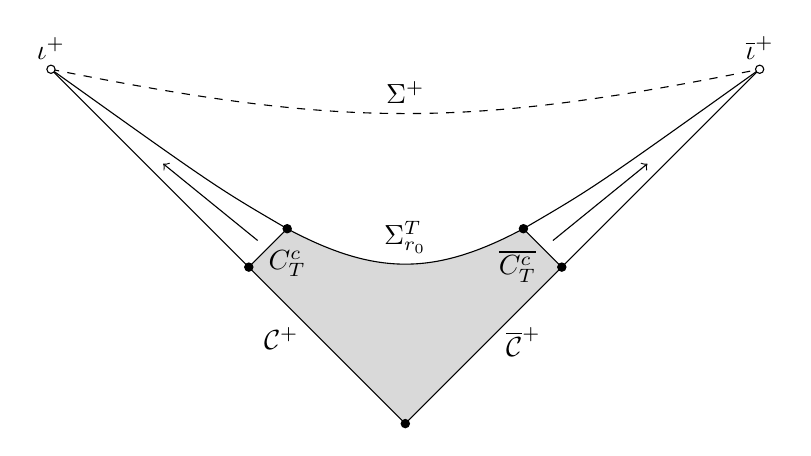
\begin{tikzpicture}[scale=1.5]
\filldraw[fill=gray!30](4.325,1.325) -- (3,0) -- (1.675,1.325) -- (2,1.65).. controls (2.75,1.25) and (3.25,1.25) .. (4,1.65) -- cycle;
\draw (0,3) -- (1.675,1.325);
\draw (4.325,1.325) -- (6,3);
\draw[dashed] (0,3) .. controls (2.5,2.5) and (3.5,2.5) .. (6,3);

\draw (3,1.8) node[below]{$\Sigma_{r_0}^T$};
\draw (2,1.65) .. controls (1.4,2) .. (0,3);
\draw (4,1.65) .. controls (4.6,2) .. (6,3);
\filldraw  (2,1.65) circle (0.035cm);
\filldraw  (1.675,1.325) circle (0.035cm);
\filldraw  (4,1.65) circle (0.035cm);
\filldraw  (4.325,1.325) circle (0.035cm);
\filldraw  (3,0) circle (0.035cm);
\draw (2,1.55) node[below]{$C_T^c$};
\draw (3.95,1.55) node[below]{$\ol{C_T^c}$};
\draw[->] (1.75,1.55) -- (0.95,2.2);
\draw[->] (4.25,1.55) -- (5.05,2.2);
\draw (3,2.8) node{$\Sigma^+$};
\draw (1.95,0.9) node[below]{$\mc{C}^+$};
\draw (4,0.9) node[below]{$\ol{\mc{C}}^+$};
\filldraw[fill=white] (0,3) circle (0.035cm);
\filldraw[fill=white] (6,3) circle (0.035cm);
\draw (0,3) node[above]{$\iota^+$};
\draw (6,3) node[above]{$\ol{\iota}^+$};
\end{tikzpicture}

\end{document}